\documentclass[conference]{IEEEtran}
\IEEEoverridecommandlockouts
% The preceding line is only needed to identify funding in the first footnote. If that is unneeded, please comment it out.
\usepackage{cite}
\usepackage{amsmath,amssymb,amsfonts}
\usepackage{algorithmic}
\usepackage{graphicx}
\usepackage{textcomp}
\usepackage{xcolor}
\usepackage{tabularray}
\usepackage{multirow}
\usepackage{multicol}
\usepackage{balance}
\def\BibTeX{{\rm B\kern-.05em{\sc i\kern-.025em b}\kern-.08em
    T\kern-.1667em\lower.7ex\hbox{E}\kern-.125emX}}

% \newcommand{\kr}[1]{\textcolor{red}{Kiran - #1}}
% \newcommand{\ku}[1]{\textcolor{violet}{Kishor - #1}}
% \newcommand{\as}[1]{\textcolor{cyan}{Anjali - #1}}

\makeatletter

\def\ps@IEEEtitlepagestyle{%
  \def\@oddfoot{\mycopyrightnotice}%
  \def\@evenfoot{}%
}
\def\mycopyrightnotice{%
  {\footnotesize TBD~\copyright~2023 IEEE\hfill}
  \gdef\mycopyrightnotice{}
}
\begin{document}

% \title{Conference Paper Title*\\
% {\footnotesize \textsuperscript{*}Note: Sub-titles are not captured in Xplore and
% should not be used}
% \thanks{Identify applicable funding agency here. If none, delete this.}
% }

\author{\IEEEauthorblockN{Hiren Vaghela\textsuperscript{1}, Anjali Sarvaiya\textsuperscript{1}, Pranav Premlani\textsuperscript{1}, Abhishek Agarwal\textsuperscript{1}, Kishor Upla\textsuperscript{1},\\ Kiran Raja\textsuperscript{2} and Marius Pedersen\textsuperscript{2}\\}
\IEEEauthorblockA{\textit{\textsuperscript{1}Sardar Vallabhbhai National Institute of Technology (SVNIT), Surat, India.}\\
\textit{\textsuperscript{2}Norwegian University of Science and Technology (NTNU), Gjøvik, Norway.}\\
{(hvaghela429, anjali.sarvaiya.as, pranavpremlani2002, abhishekag2702, kishorupla)}@gmail.com\\
{(kiran.raja, marius.pedersen)}@ntnu.no
}
}
\title{DCAN:DenseNet with Channel Attention Network for Super-resolution of Wireless Capsule Endoscopy}
\maketitle
% Wireless Capsule Endoscopy Image Super Resolution using Deep Learning
\begin{abstract}
Wireless Capsule Endoscopy (WCE) captures images of the gastrointestinal (GI) tract and transmits the images in a wireless manner. Due to the hardware limitations of the capsule and the varying imaging conditions within the GI tract, the recorded images can have a low spatial resolution with a high frame rate or a high spatial resolution with a low frame rate. Although it is generally common to have low spatial resolution to capture details of the GI tract, low spatial resolution limits the detection of minor anatomical features and abnormalities in the small intestine and other portions of the GI tract. Super-Resolution (SR) is a class of software-based techniques that are used to enhance the resolution of a Low-Resolution (LR) image. This work proposes a new model referred as \emph{DCAN}-DenseNet with Channel Attention Network for Super-resolution of LR WCE images. The design of \emph{DCAN} consists of multiple strategies adopted from state-of-the-art methods such as Channel Attention Network (CAN) from RCAN and short dense connections from DenseNet to extract details from LR observation. Additionally, to improve the accuracy of the SR images, we create a derivative dataset of 10,000 images from a publicly available WCE dataset. The proposed approach has been validated against multiple state-of-the-art methods by conducting quantitative evaluation using perceptual metrics. 
The analysis is complemented by statistical validation to demonstrate the consistency of the proposed method over the other models for the SR task.

\end{abstract}

\begin{IEEEkeywords}
Wireless Capsule Endoscopy, Super Resolution, Channel Attention Network, DCAN
\end{IEEEkeywords}

\section{Introduction}
The Wireless Capsule Endoscopy (WCE) is a minimally invasive medical technology that utilizes a small, swallowable capsule equipped with a wireless camera to capture images and videos of GastroIntestinal (GI) tract. Captured video frames are transmitted to a recording device outside the patient's body. It allows for a comprehensive examination of the small intestine similar to conventional endoscopy but with additional convenience. The recorded images and videos provide valuable diagnostic information about GI disorders such as Crohn's disease, tumors, bleeding, or Inflammatory Bowel Disease (IBD) \cite{WCE}. It generates an average of 50k to 60k images while moving through the GI tract, and a normal colon video test generates about 8 hours of RGB video data. Thus, the vast amount of data generated by WCE presents a challenge for medical professionals, who must verify numerous images or videos. Continued advancements in technology and image analysis algorithms further enhance the capabilities of WCE, leading to improved patient care and outcomes.

Resolution plays a crucial role in all vision-driven applications including medical diagnosis. A low resolution video/image can lead to incorrect diagnostics for both machines and medical practitioners \cite{WCE2}. The image sensor equipped with High-Resolution (HR) can help visualise intricate details within the digestive tract, such as mucosal irregularities, ulcers, polyps, or early-stage tumors \cite{WCE3}. The clear and detailed images obtained from HR camera allowing doctors for targeted interventions or surgical procedures. However, a capsule consisting of an optical dome, illuminator, imaging sensor, battery, and RF transmitter in a capsule-shaped structure with a length of 26 mm and a diameter of 11 mm \cite{WCE} can work in two modes. The small-sized structure leads to hardware limitations in terms of spatial resolution of sensor which is usually coarser. The minimum resolution obtained by a capsule used is $336 \times 336$ pixels with 24 frames per second (fps) \cite{data} and the maximum resolution of 1 megapixel can reduce the frames rate to 5 fps. Having higher fps is advantageous in covering large area and despite of having numerous benefits of WCE technology, the operational fps suffers from inadequate frame resolution and video quality leading to adverse diagnostics \cite{lowres}. Thus, there is a clear demand for methods capable of enhancing the resolution of capsule endoscopes to facilitate both subjective and objective analysis.


Image Super-Resolution (SR) is a software-driven method used to enhance the LR image to its corresponding HR one. Single Image SR (SISR) and Multi-Image Super-Resolution (MISR) are the two types of SR methods, with SISR being more popular due to its advantages over MISR, where multiple images of the same scene and image registration are required. However, SISR poses a challenging ill-posed problem as a single LR image may correlate to several HR solutions \cite{SISR}. The recent advancement of deep learning techniques has resulted in a number of techniques that can be used in SISR making it possible to use for other applications.


Inspired by the success of applications in other domains, we present a SR approach for WCE images using a deep learning-based approach which we refer to as \emph{DCAN}-DenseNet with Channel Attention Network (CAN). The proposed architecture incorporates the CAN mechanism for extracting high-level details by feature scaling in an adaptive way. Such a mechanism allows us to leverage the high frequency details in WCE image to identify and retain abnormality present in the WCE images for downstream classification tasks like pathology classification. Additionally, we also introduce short skip connections to extract low-level features that are common in images from the GI tract. The low level features are then combined with the high-level features to generate information-rich SR images. To enhance the reconstruction process and recover image details, we also employ bottleneck, deconvolution, and reconstruction layers. The potential of the proposed model is evaluated on a new derived dataset created from the original Kvasir capsule endoscopy dataset \cite{data}. Our contributions from this work are:
\begin{itemize}
    \item A new SR approach that leverages Channel Attention Network (CAN) and Dense connections to generate SR images from LR images. 
%    
    \item The CAN in the proposed model adaptively re-scales the features by taking into account the inter-dependencies among different features. Further, the use of short skip connections in convolution layers specializes in excessing the high-level features to obtain low-level features in the input LR image, which is important for better detailing in reconstruction of the SR image. 
    
    \item Unlike other approaches, we propose training and testing of WCE images in the $Y$-channel of $YCbCr$ which provides better performance metrics compared to RGB color scheme and corresponds closely to the Human Visual System (HVS). This is validated through empirically through various metrics such as Peak Signal to Noise Ratio (PSNR), Structural Similarity Index Metric (SSIM) and Learned Perceptual Image Patch Similarity (LPIPS) which asserts our intuition of using $YCbCr$ over RGB processing. 
    \item Further, due to unavailability of datasets for SR tasks, we create a new derivative dataset from Kvasir Capsule Endoscopy \cite{data} to train the SR network. The new dataset consists of 10,000 samples which are manually pre-processed to improve the accuracy of the proposed network. All our experiments are conducted using state-of-the-art methods to demonstrate the applicability of proposed approach for SR generation and is supported by detailed analysis of various perceptual metrics.
\end{itemize}




\section{Literature Review} 

 SR methods based on deep learning aim to capture the complex relationship between given LR and HR images. Dong et al. \cite{SRCNN} introduced Super-resolution Convolutional Neural Network (SRCNN) consisting shallow network of having 3 layers. Later, Kim et al. increased the network depth to 20-layers proposed VDSR \cite{VDSR} and DRCN \cite{DRCN}, which achieved notable improvements over the previous SRCNN indicating the importance of network depth. In similar lines, Lim et al.\cite{EDSR} further advanced this concept by creating the EDSR, a very wide network an exceptionally deep network consisting of approximately 165 layers, using simplified residual blocks. However, it is worth noting that merely stacking residual blocks to construct deeper networks does not necessarily lead to significant improvements. 

Tong et al. introduced DenseNet \cite{SRDensenet} leveraging dense connections between convolution layers and growth rate to quantify the amount of new information added by each layer to the final reconstruction. Also due to dense connections all level of high, average and low level of features can be extracted easily. Thus, the DenseNet model utilizes feature maps from each layer that are merged with the previous layer, and the data is replicated multiple times for effective training of very deep networks. Zhang at el. proposed RCAN \cite{RCAN} model with Residual in Residual (RIR) structure where the Residual Group (RG) acts as the basic module and allows for residual learning in a coarse level through the use of Long Skip Connections (LSCs). This model also introduces a Channel Attention (CA) mechanism, which adaptively re-scales each channel-wise feature by modeling the inter-dependencies across feature channels. This mechanism enables the network to focus on more useful channels, thereby enhancing its discriminative learning ability. Several other SR works have been proposed to enhance the perceptual quality of SR results. For instance, Ledig et al. \cite{SRGAN} proposed an SRGAN model that improves the perceptual quality of super-resolved images beyond pixel-level improvements. Similarly, Wang et al. \cite{ESRGAN} proposed an Enhanced Super Resolution using GAN (ESRGAN), which introduces several improvements over SRGAN. These works have been tested on visible (i.e., RGB scene) images and are also extended to medical data. Mahapatra et al. in \cite{L10} used Progressive GAN (P-GAN) for accurate detection and proper segmentation of anatomical landmarks on MRI images. Additionally, a few other SR techniques have also been utilized to improve the quality of images acquired by traditional endoscopic cameras. Yasin et al. \cite{EndoL2H} learned a mapping from low-to-high resolution mapping using conditional adversarial networks with a spatial attention block to improve the resolution by up to factors of $\times 8$, $\times 10$, $\times 12$ respectively. However, the approach is limited to conventional endoscopy images. Thus, the super-resolution of WCE images is not attempted by researchers in the community to the best of our knowledge motivating us to focus on SR task for WCE images.


\section{Proposed method: DenseNet with Channel Attention Network (DCAN)}
With the aim of recovering rich high-frequency details from capsule endoscopy images, the proposed approach consists design inspired from RCAN \cite{RCAN} and DenseNet \cite{SRDensenet}. The RCAN model is one of the state-of-the-art methods for SR of visible images which has introduced novel Channel Attention Network (CAN) to improve the learning ability of CNN network. Similarly, dense connections are usually employed in the CNN network to learn effective features from LR images and also to reduce the effect of overfitting or underfitting.  Motivated by these, we incorporated the above concepts in the proposed method which we referred as \emph{DCAN}-DenseNet with Channel Attention Network. In WCE images, low-frequency components display a relatively homogeneous pattern, the high-frequency elements typically correspond to regions characterized by edges, texture, and other intricate details. Thus, the use of CAN in the proposed model enhances channel-wise feature representations, and hence, \emph{DCAN} gains the advantage to extract information more precisely. The fusion of this with dense connections results in a powerful architecture that leverages the strengths of both RCAN and DenseNet, enabling it to effectively handle the task at hand and achieve superior performance in acquiring intricate details within WCE data. 


\begin{figure*}[t!]
    \centering
    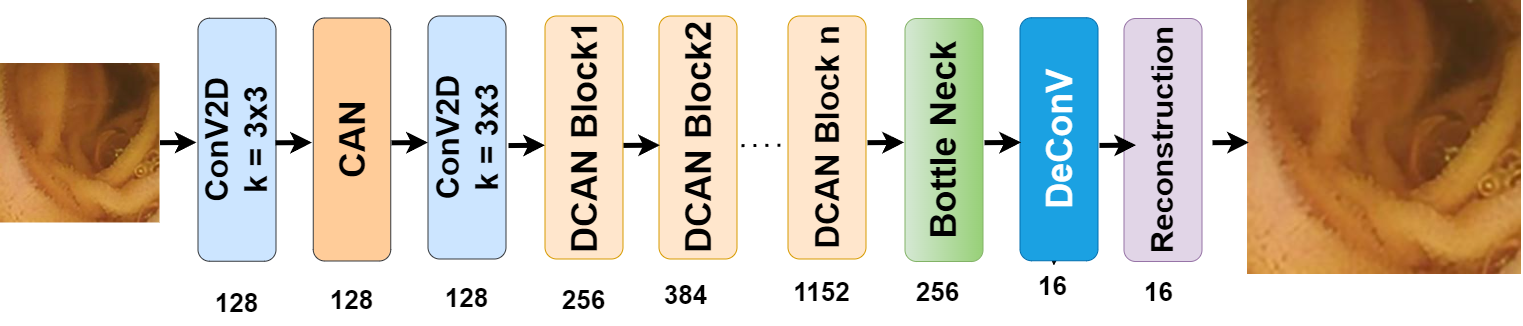
\includegraphics[width=0.99\textwidth]{1_fff.drawio.png} 
    \caption{The network architecture of proposed model \emph{DCAN}, where $k$ denotes kernel size and numerical values mentioned below every layer indicates size of output features.}
    \label{fig:label6.8}
\end{figure*}
The architecture of the proposed model for the task of SR of WCE images for upscaling factors $\times 4$ is depicted in Fig.~\ref{fig:label6.8}. It can be observed that the WCE LR image is given to a convolution layer first to learn low-level features. After this, a single CAN layer is added to learn the features channel wise from the LR image. Subsequently, a series of DCAN blocks are employed to learn high-level features. Towards the end, the bottleneck layer is used to decrease the input feature maps and finally, the deconvolution layer is employed to upsample the feature images, and the output of the reconstruction layer generates an SR image.
 
\begin{figure}[h!]
    \centering
    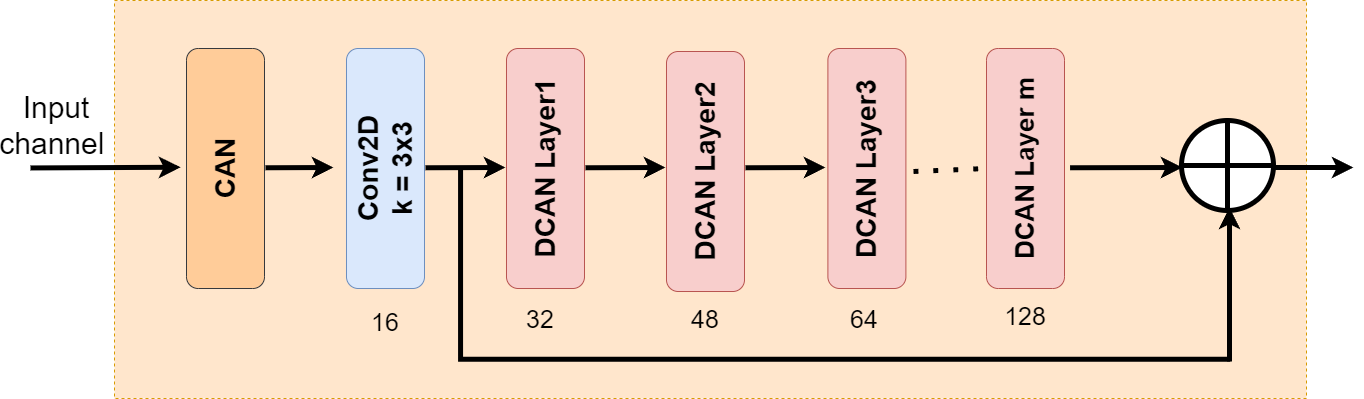
\includegraphics[width=0.5\textwidth]{2.drawio (4).png} %[totalheight=1.2in]
    \caption{The network architecture of DCAN block used in proposed model-\emph{DCAN}. The values below every layer indicate the number of output features.}
    \label{fig:label6.9}
\end{figure}
\subsection{DCAN Block}
In the proposed network, we utilize DCAN blocks as fundamental building unit. This design allows to enhance details and promotes feature reuse throughout the network, leading to more comprehensive and expressive representations at higher layers. The network architecture of DCAN block is depicted in Fig.~\ref{fig:label6.9}. There are $n$ number of DCAN blocks used in our architecture, which we fix to $8$ empirically. Each DCAN block consists of Channel Attention Network (CAN), one convolution layer and $m$ number of DCAN layers (i.e., $m=8$) that enable to extract high-level features in the output image. Moreover, one skip connection is added to avoid vanishing-gradient problem. The block schematic DCAN layer is shown in Fig.~\ref{fig:label6.10} (a). Each DCAN layer consists of a convolution layer having kernel size $3\times3$ and Relu activation function with short skip connection. Thus, the proposed model consists of short skip connections and also global skip connections for effective learning and also to avoid gradient problem. 



\begin{figure}[h!]
    \centering
    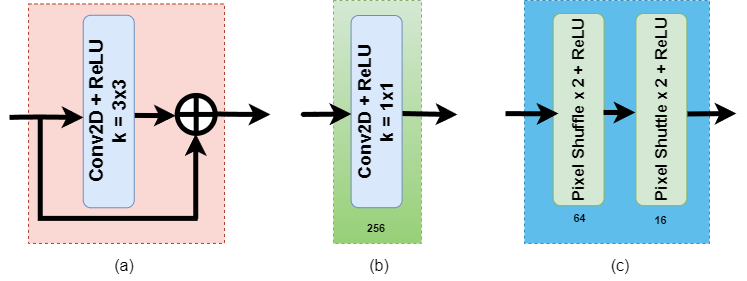
\includegraphics[width=0.5\textwidth]{fi.drawio (2).png} % [totalheight=1.2in]
    \caption{The design of (a) DCAN Layer, (b) Bottleneck Layer and (c) Deconvolution Layer in the proposed method.}
    \label{fig:label6.10}
\end{figure}

\subsection{Channel Attention Network (CAN)}
The earlier CNN-based SR methods \cite{SRCNN, VDSR, DRCN, ResNet, EDSR, SRDensenet}, treat LR channel-wise features equally, which is not optimal for real-world cases. To address this issue and focus the network on more informative features, CAN mechanism is proposed in RCAN \cite{RCAN} that exploits the interdependencies among feature channels. Generating different attention for each channel-wise feature is a crucial step in this mechanism. An LR information contains both low-frequency and high-frequency components that are valuable for SR. However, the low-frequency parts are relatively homogeneous, while the high-frequency components typically correspond to regions with edges, texture, and other details. Second, each filter in the convolution layer operates within a local receptive field, which limits its ability to exploit contextual information beyond the local region. Thus, the use of CA in the proposed method is helpful to learn the features effectively by assigning proper weights to each feature. The architecture for CAN is depicted in Fig.~\ref{fig:label6.11}. It consists of adaptive average pooling with a convolution layer with kernel size $3\times3$, attached with a ReLU activation function, which is passed to another convolution layer with kernel $1\times1$, and a skip connection is used to add the input values with the output of the sigmoid function.
\begin{figure}[h!]
    \centering
    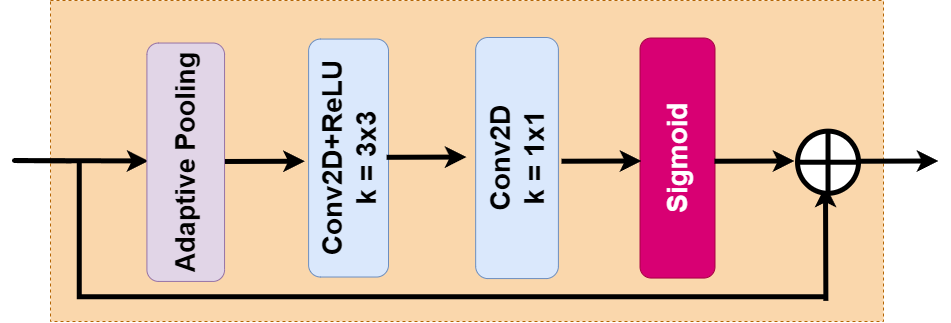
\includegraphics[width=0.5\textwidth]{4.drawio_fff.png} % [totalheight=1.2in]
    \caption{The architecture design of Channel Attention Network (CAN) used in \emph{DCAN} model.}
    \label{fig:label6.11}
\end{figure}


\subsection{BottleNeck Layer}
In order to enhance the compactness and computational efficiency of the model, we use a bottleneck layer to decrease the quantity of feature maps prior to their input into the deconvolution layers. The bottleneck layer shown in Fig.~\ref{fig:label6.10}(b) is used to reduce the output features from DCAN blocks to a lower dimension. It consists of a convolution layer having kernel size $1\times1$ with ReLU activation function. In our proposed model, we reduce the features to 256 features using the bottleneck layer. 

\subsection{Deconvolution and Reconstruction Layers}
Deconvolution layers can be seen as the inverse operation of convolution layers, allowing for the learning of diverse upscaling kernels that work together to predict HR images. It provides two advantages: By conducting computations in the LR space, the SR reconstruction process is accelerated. %This approach significantly reduces the computational cost by a factor equal to the square of the upsampling factor employed. 
Additionally, the inclusion of a deconvolution layer enables the utilization of contextual information from LR images to infer high-frequency details.
The network design of the Deconvolution layer consists of two pixel-shuffle layers as shown in Fig.~\ref{fig:label6.10}(c), where each layer upsamples the image by a factor of $\times2$. Pixel-shuffle rearranges the feature maps by reshaping them into a higher resolution. Then it rearranges the pixel values to get the final image. We are using two pixel-shuffle layers which give us total  upsampling of factor $4$. 
Finally, a reconstruction layer, consisting of a convolution layer with a $3\times3$ kernel, is used to generate SR images from the feature maps in the RGB space.



\begin{figure*}[!t]
    % \centering
    % \includegraphics[totalheight=1.2in]{520_final_result.png}
    % \caption{Deconvolution Layer}
    % \label{fig:label6.12}
    % \centering
    % \begin{subfigure}
    %     \includegraphics{520/520_box.png}
    % \end{subfigure}
    % \hfill
    % \begin{subfigure}[b]{0.3\textwidth}
    %     \centering
    %     \includegraphics{520/520_bicubic.jpg}
    %     \caption{Bicubical}
    %     \vfill
    %     \includegraphics{520/520_Bicubical_ssim.jpg}
    %     \caption{Bicubical kernel}
    % \end{subfigure}
    \minipage{0.24\textwidth}
        \centering
        \includegraphics[width=\linewidth]{Figures/520/520_box.png}
    
    \endminipage\hfill
    \minipage{0.12\textwidth}
        \centering
        \includegraphics[width=\linewidth]{Figures/520/520_bicubic.jpg}
        
        \vfill
        \includegraphics[width=\linewidth]{Figures/520/520_Bicubical_ssim.jpg}
         
    \endminipage\hfill
    \minipage{0.12\textwidth}
        \centering
        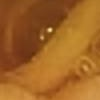
\includegraphics[width=\linewidth]{Figures/520/520_SRGAN.jpg}
        
        \vfill
        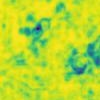
\includegraphics[width=\linewidth]{Figures/520/520_SRGAN_ssim.jpg}
        
    \endminipage\hfill
    \minipage{0.12\textwidth}
        \centering
        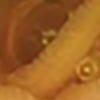
\includegraphics[width=\linewidth]{Figures/520/520_cycleGAN.jpg}
        
        \vfill
        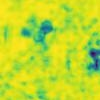
\includegraphics[width=\linewidth]{Figures/520/520_cycleGAN_ssim.jpg}
        
    \endminipage\hfill
    \minipage{0.12\textwidth}
        \centering
        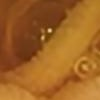
\includegraphics[width=\linewidth]{Figures/520/520_Densenet.jpg}
        
        \vfill
        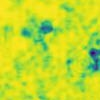
\includegraphics[width=\linewidth]{Figures/520/520_DenseNet__ssim.jpg}
        
    \endminipage\hfill
    \minipage{0.12\textwidth}
        \centering
        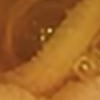
\includegraphics[width=\linewidth]{Figures/520/520_RCAN.jpg}
       
        \vfill
        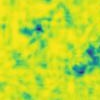
\includegraphics[width=\linewidth]{Figures/520/520_RCAN_ssim.jpg}
        
    \endminipage\hfill
    \minipage{0.12\textwidth}
        \centering
        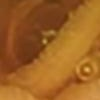
\includegraphics[width=\linewidth]{Figures/520/520_proposed.jpg}
        
        \vfill
        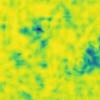
\includegraphics[width=\linewidth]{Figures/520/520_proposed_ssim.jpg}
        
    \endminipage\hfill
    %\caption{Patch analysis of images on different models using perceptual technique and attention maps }

\minipage{0.24\textwidth}
        \centering
        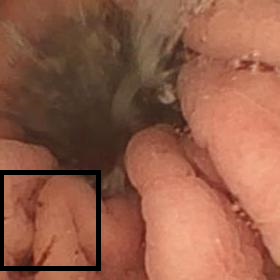
\includegraphics[width=\linewidth]{Figures/906/906_border.png}
        
    \endminipage\hfill
    \minipage{0.12\textwidth}
        \centering
        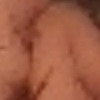
\includegraphics[width=\linewidth]{Figures/906/906_Bicubical.jpg}
        
        \vfill
        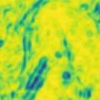
\includegraphics[width=\linewidth]{Figures/906/906_Bicubical_ssim.jpg}
        
    \endminipage\hfill
    \minipage{0.12\textwidth}
        \centering
        
\includegraphics[width=\linewidth]{Figures/906/906_SRGAN.jpg}
        
        \vfill
        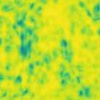
\includegraphics[width=\linewidth]{Figures/906/906_SRGAN_ssim.jpg}
        
    \endminipage\hfill
    \minipage{0.12\textwidth}
        \centering
        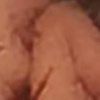
\includegraphics[width=\linewidth]{Figures/906/906_cycleGAN.jpg}
        
        \vfill
        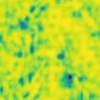
\includegraphics[width=\linewidth]{Figures/906/906_cycleGAN_ssim.jpg}
        
    \endminipage\hfill
    \minipage{0.12\textwidth}
        \centering
        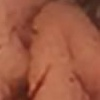
\includegraphics[width=\linewidth]{Figures/906/906_Densenet.jpg}
        
        \vfill
        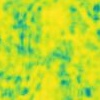
\includegraphics[width=\linewidth]{Figures/906/906_densenet_ssim.jpg}
        
    \endminipage\hfill
    \minipage{0.12\textwidth}
        \centering
        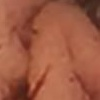
\includegraphics[width=\linewidth]{Figures/906/906_RCAN.jpg}
        
        \vfill
        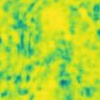
\includegraphics[width=\linewidth]{Figures/906/906_RCAN_ssim.jpg}
        
    \endminipage\hfill
    \minipage{0.12\textwidth}
        \centering
        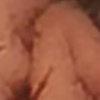
\includegraphics[width=\linewidth]{Figures/906/906_proposed.jpg}
        
        \vfill
        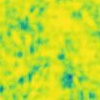
\includegraphics[width=\linewidth]{Figures/906/906_proposed_ssim.jpg}
        
    \endminipage\hfill
   % \caption{Patch analysis of images on different models using perceptual technique and attention maps }

\minipage{0.24\textwidth}
        \centering
        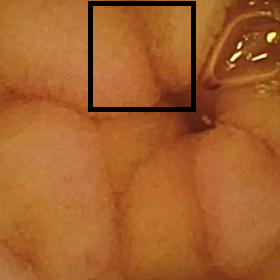
\includegraphics[width=\linewidth]{Figures/983/983_box.png}
        HR
    \endminipage\hfill
    \minipage{0.12\textwidth}
        \centering
        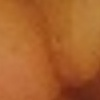
\includegraphics[width=\linewidth]{Figures/983/983_Bicubical.jpg}
         \\
        \vfill
        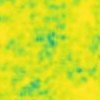
\includegraphics[width=\linewidth]{Figures/983/983_Bicubic__ssim.jpg}
        Bicubic \\
    \endminipage\hfill
    \minipage{0.12\textwidth}
        \centering
        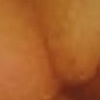
\includegraphics[width=\linewidth]{Figures/983/983_SRGAN.jpg}
         \\
        \vfill
        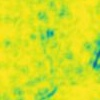
\includegraphics[width=\linewidth]{Figures/983/983_SRGAN__ssim.jpg}
        SRGAN \\
    \endminipage\hfill
    \minipage{0.12\textwidth}
        \centering
        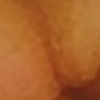
\includegraphics[width=\linewidth]{Figures/983/983_cycleGAN.jpg}
         \\
        \vfill
        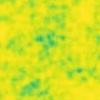
\includegraphics[width=\linewidth]{Figures/983/983_cycleGAN_ssim.jpg}
        CycleGAN \\
    \endminipage\hfill
    \minipage{0.12\textwidth}
        \centering
        
\includegraphics[width=\linewidth]{Figures/983/983_DenseNet.jpg}
         \\
        \vfill
        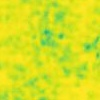
\includegraphics[width=\linewidth]{Figures/983/983_densenet_ssim.jpg}
        DenseNet\\
    \endminipage\hfill
    \minipage{0.12\textwidth}
        \centering
        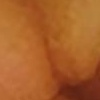
\includegraphics[width=\linewidth]{Figures/983/983_RCAN.jpg}
        \\
        \vfill
        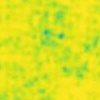
\includegraphics[width=\linewidth]{Figures/983/983_RCAN_ssim.jpg}
        RCAN\\
    \endminipage\hfill
    \minipage{0.12\textwidth}
        \centering
        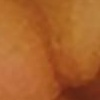
\includegraphics[width=\linewidth]{Figures/983/983_proposed.jpg}
      
        \vfill
        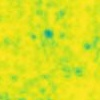
\includegraphics[width=\linewidth]{Figures/983/983_proposed_ssim.jpg}
        Proposed
    \endminipage\hfill
    \caption{Qualitative comparision of proposed models with state-of-the-art models using SSIM maps (where yellow region shows similarity and blue region shows disimilarity.)}
    \label{fig:qualanal}
\end{figure*}

\section{Experimental Analysis}
The design of the proposed model is validated by conducting subjective and quantitative evaluations. We empirically verify DCAN’s effectiveness %on a chosen dataset of 1000 images and compare% 
with state-of-the art architectures qualitatively by taking a patch from the output images from all state-of-the-art models. Additionally, the same is quantitatively verified using different standard SR metrics such as Peak Signal to Noise Ratio (PSNR) \& Structural Similarity Index Metric (SSIM) and using perceptual metric i.e., Learned Perceptual Image Patch Similarity (LPIPS).  Finally, the statistical analysis of the proposed model is also carried out to show the consistency of the SR results. Our method is benchmarked against state-of-the-art models such as SRGAN \cite{SRGAN}, CycleGAN \cite{CycleGAN}, DenseNet \cite{SRDensenet}, and RCAN \cite{RCAN} for comparison purposes.  
\subsection{Dataset}
One of the novel contributions of the work is the creation of new derivative dataset from the available Kvasir Capsule Endoscopy Dataset \cite{data} consisting of WCE images.  
%The dataset consists of a  segment of Kvasir-Capsule, a video capsule endoscopy dataset.  \textbf{}  in \emph{Supplementary material} due to space constraints
In the original Kvasir dataset, each image is in the RGB color space with size of $336\times336$ pixels. The dataset contains a total of $47,236$ images, which are categorized according to different medical anomalies. As the original dataset contained redundant images with many border areas with black pixels, we have curated the dataset for the SR task by manually selecting images and removing redundant images from the Kavasir dataset.  
The new SR dataset therefore consists of $10,000$ training images, $550$ validation images and $1000$ testing images \footnote{The dataset will be made available for researchers provide they have license agreement for original Kvasir Capsule dataset.}. As mentioned earlier, the WCE images from the original Kvasir dataset containing non-informative part in the border area. Those regions are removed manually through cropping resulting in images of $280\times280$ pixels for all images. The proposed model along with all other models are experimented on the new datset and SR results are generated.


\subsection{Training details}
Firstly, to prepare LR-HR pair of WCE images, we consider the original images as the HR image and applied bicubic down-sampling with factor $\times 4$ and obtained LR image. These LR-HR pairs are fed to the proposed model to train it to generate SR images. Further, each LR image has also been transformed into $YCbCr$ space and only the $Y$-channel was used for training which represents a gamma-encoded channel that predominantly contains high-level feature information. On the other hand, the Cb and Cr channels are chroma-encoded channels that do not contain as many high-level features. To save computational time during the process and improve the extraction of high-level features in the SR image, the Cb and Cr channels are directly interpolated and added to the output image. The training process aimed to minimize the loss function, which was taken as the Mean Squared Loss (MSE). The training was carried out for a total of $300$ epochs with a batch size of $32$. Additionally, the Adam optimizer was used with a learning rate of $0.0001$. This protocol was used on all the state-of-the-art models and SR results are generated. While testing, we use the YCbCr space of test LR image to generate the SR image.



\subsection{Comparison with state-of-the-art models}

\textit{Qualitative Analysis:}
The qualitative comparison of various SR methods on scaling factor of $\times4$ is depicted in Fig.~\ref{fig:qualanal}. One can inspect by looking at the zoomed-in patches that the proposed model generates better SR solutions than other models. Also, the SSIM map of each patch is shown below the patch SR image, which shows the similarity between generated SR and HR images. The yellow part in the SSIM maps shows the similarity between SR and HR images. However, the green and blue regions in SSIM maps show the dissimilarity between SR and HR images. We can observe that the proposed model has more similar parts than the other methods.  In the first row SSIM maps in Fig.~\ref{fig:qualanal}, it can be observed that the bicubic output image exhibits the highest dissimilarity. Comparatively, other models such as RCAN and DenseNet perform better than other models as well as the bicubic method. However, the proposed model demonstrates the lowest dissimilarity among the bicubic method and all other state-of-the-art models. Additionally, in the second row, it is apparent that SRGAN and DenseNet exhibit better performance in comparison. However, the proposed model demonstrates the highest structural similarity, indicating superior performance in terms of preserving the structural characteristics of the image. 

\subsubsection*{Quantitative Analysis}
To validate the SR results quantitatively, the average SSIM and PSNR values for the testing images of each model are provided in Table~\ref{quantal}. We calculated the average PSNR and SSIM on $Y$ channel as well as the RGB channels. From the table, it can be observed that the proposed DCAN model has the highest PSNR in both the Y channel and the RGB channel. Additionally, the DCAN model also demonstrates the highest SSIM values, implying a better structural similarity. When considering LPIPS for perceptual image comparison, lower LPIPS values emphasize the model's ability to capture perceptual similarity effectively. Remarkably, the DCAN model exhibits the lowest LPIPS values among all different models, suggesting superior perceptual similarity. 

\begin{table}[h!]
\centering
\caption{Quantitative comparison of the proposed model over other models using different metrics such as PSNR, SSIM and LPIPS on RGB and Y-channels.}
\label{quantal}
\resizebox{0.49\textwidth}{!}{
\begin{tabular}{|l|cc|cc|c|}
\hline
Model & \multicolumn{2}{c|}{PSNR $\uparrow$}                                            & \multicolumn{2}{c|}{SSIM $\uparrow$}                                       & \multicolumn{1}{l|}{LPIPS$\downarrow$} \\ \cline{2-6} 
                       & \multicolumn{1}{c|}{Y-channel}        & \multicolumn{1}{c|}{RGB}     & \multicolumn{1}{c|}{Y-channel}       & \multicolumn{1}{c|}{RGB} & \multicolumn{1}{c|}{RGB}   \\ \hline
Bicubic                & \multicolumn{1}{c|}{38.1069}          & \multicolumn{1}{l|}{37.2111} & \multicolumn{1}{c|}{0.9296}          & 0.9057                   & 0.2310                     \\ \hline
SRGAN \cite{SRGAN}         & \multicolumn{1}{c|}{38.0377}          & 37.0021                      & \multicolumn{1}{c|}{0.9291}          & 0.9049                   & 0.1972                     \\ \hline
CycleGAN \cite{CycleGAN}      & \multicolumn{1}{c|}{38.0121}          & 36.9441                      & \multicolumn{1}{c|}{0.9123}          & 0.9012                   & 0.1984                     \\ \hline
DenseNet \cite{SRDensenet}   & \multicolumn{1}{c|}{39.6842}          & 38.8596                      & \multicolumn{1}{c|}{0.9401}          & 0.9369                   & 0.1353                     \\ \hline
RCAN \cite{RCAN}          & \multicolumn{1}{c|}{40.1438}          & 39.4613                      & \multicolumn{1}{c|}{0.9427}          & 0.9371                   & 0.1359                     \\ \hline
Proposed  & \multicolumn{1}{c|}{\textbf{40.2261}} & \textbf{39.5389}             & \multicolumn{1}{c|}{\textbf{0.9486}} & \textbf{0.9378}          & \textbf{0.1346}            \\ \hline
\end{tabular}
}
\end{table}

\subsubsection*{Statistical Analysis}
Finally, the statistical analysis is also conducted on the SR results of the proposed model along with the others to ensure the model consistency compared to state-of-the-art models. Standard deviation demonstrates the deviation in the values from the mean and hence it should be low for an algorithm. The values of standard deviation of each model are presented in Table~\ref{table:stanal}. As we can observe the values of our proposed model DCAN is lowest in comparision to all state-of-the-art models. From the given values, it can be noticed that while comparing PSNR consistency $Y$ channel has lower consistency than the RGB channels and while comparing SSIM, its vice-a-versa. Thus, one can conclude from this that there is high peaks in $Y$-channel i.e., $Y$-channel works great on majority images and provides better PSNR values, but as it focuses only on $Y$-channel, the features in $Cb$ and $Cr$ channels are not percieved properly, so when the high-level features are in the $Cb$ and $Cr$ channels, it loses important information which is although a rare case as all important information is in $Y$-channel majorly. %The box-plot representations of the same is discussed in \emph{Supplementary material} due to space constraints. 



\begin{table}[]
\centering
\caption{The statistical comparison of the proposed model with other different methods using parameter of Standard Deviation of PSNR and SSIM values over mean values in RGB and Y-channels.}
\label{table:stanal}
\begin{tabular}{|l|cc|cc|c|}
\hline
Model & \multicolumn{2}{c|}{STD. dev. of PSNR $\downarrow$}                                            & \multicolumn{2}{c|}{STD. dev. of SSIM $\downarrow$}            \\ \cline{2-5} 
                       & \multicolumn{1}{c|}{Y-channel}        & \multicolumn{1}{c|}{RGB}     & \multicolumn{1}{c|}{Y-channel}       & \multicolumn{1}{c|}{RGB} \\ \hline
Bicubic                & \multicolumn{1}{c|}{3.8943}          & \multicolumn{1}{l|}{2.2102} & \multicolumn{1}{c|}{0.0353}          & 0.0347                  \\ \hline
SRGAN \cite{SRGAN}                 & \multicolumn{1}{c|}{3.3490}          & 2.6924                     & \multicolumn{1}{c|}{0.0348}          & 0.0324                                    \\ \hline
CycleGAN \cite{CycleGAN}              & \multicolumn{1}{c|}{3.6802}          & 2.1937                     & \multicolumn{1}{c|}{0.0356}          & 0.0319                                     \\ \hline
DenseNet \cite{SRDensenet}             & \multicolumn{1}{c|}{4.2025}          & 3.1996                      & \multicolumn{1}{c|}{0.0378}          & 0.0372                                    \\ \hline
RCAN  \cite{RCAN}                 & \multicolumn{1}{c|}{3.5612}          & 2.8753                      & \multicolumn{1}{c|}{0.0367}          & 0.0350                                \\ \hline
Proposed               & \multicolumn{1}{c|}{\textbf{3.0006}} & \textbf{2.0186}             & \multicolumn{1}{c|}{\textbf{0.0270}} & \textbf{0.0306}                    \\ \hline
\end{tabular}
\end{table}



\section{Conclusion}
%In this paper, we address the super-resolution of WCE images. 
Due to the hardware limitations of the WCE sensors, the captured data results in coarser resolution which affects the diagnosis accuracy of the diseases. We present a new SR approach \emph{DCAN} using dense connections and channel attention modules to convert LR images to SR images. As the proposed network integrates the advantages of Channel Attention Network (CAN) from RCAN and utilizes short dense connections inspired by DenseNet, the proposed approach is able to effectively extract details from LR observations. Experiments show that the proposed  network can perform better than other  existing state-of-the-art SR models both quantitatively and qualitatively. The results are supported with a detailed analysis of quality assessment metrics such as PSNR, SSIM, and LPIPS and statistical analysis of obatained results. A future direction in this work is to focus on improving the perceptual quality and assess it with medical practitioners. 

\section*{Acknowledgment}
Authors are thankful to Research Council of Norway (RCN) for International Network for Capsule Imaging in Endoscopy (CapsNetwork) project managed by Department of computer science, Norwegian University of Science and technology (NTNU), Norway for providing support for this research work.


\balance
\bibliographystyle{ieeetr}
\bibliography{./IEEEabrv,mybibfile}
\end{document}